%% PARTIE 5 : Architecture et Algorithmes

Plug-in mis à part, l'exécutable est organisé autour de trois modules principaux : \texttt{Parser}, \texttt{Solver} et \texttt{Outer}, qui servent respectivement à convertir un fichier SVG en notre représentation interne, à traiter cette représentation et à effectuer la conversion inverse, la classe \texttt{Solver} étant abstraite (elle implémente le packer identité) et permettant la création de "sous-solveurs" par héritage.\\

Les modules communiquent entre eux comme indiqué en figure~\ref{ps}.

\begin{figure}[hbt!]
\center
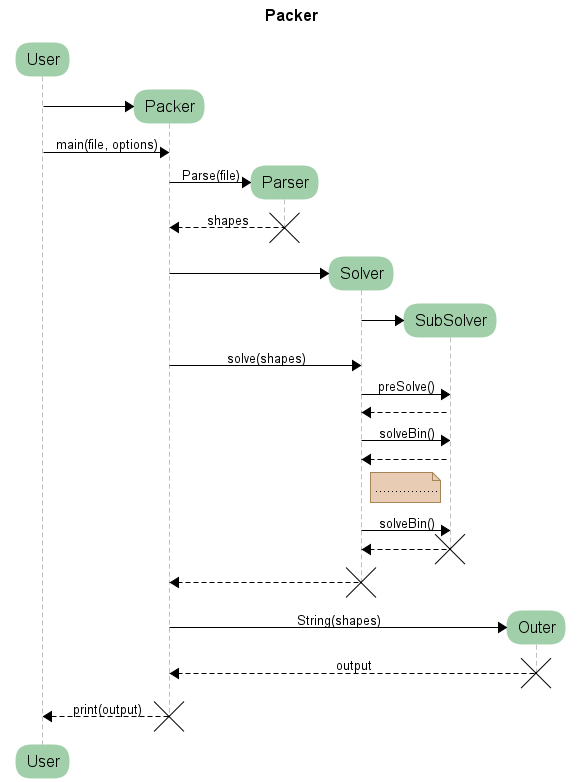
\includegraphics[scale=0.7]{img/packerSeq}
\caption{Diagramme de séquences du cas d'utilisation nominal}
\label{ps}
\end{figure}
\newpage
\subsection{Parser}

\texttt{SVG++} est utilisé comme aide au parsing : à l'aide de \texttt{rapidXML}, le fichier contenant les formes est lu sous forme d'arbre xml, puis il passe les informations qu'il parse à notre programme. Le nom des méthodes pour recevoir les informations de parsing est prédéfini, le code de chacune d'entre elle est alors à définir dans notre classe de \texttt{parseur} : il faut définir pour chaque type de balise SVG les actions à réaliser à l'entrée sur celles-ci (et potentiellement à la sortie) et les informations à stocker pour effectivement parser notre document.\\

\indent Les informations que nous cherchons à acquérir sont tout principalement les formes à packer, cependant nous avons également besoin de stocker d'avantage d'information pour effectuer un packing efficace, notamment les dimensions du document qui correspondent dans le cas ou cette information n'est pas passée en paramètre à la taille de la plaque sur laquelle réaliser le traitement.\\

\indent D'autres contraintes de fidélité nous poussent à gérer séparément d'autres informations telles que les matrices de transformation déjà présentes dans le fichier, et les groupes correspondant à des ensembles de pièces atomiques (par exemple une pièce trouée).\\


\indent Le dernier problème à s'être posé lors de la lecture du fichier est la présence de matrices de transformations dans les attributs des objets, des objets englobant plusieurs pièces tels que les groupes pouvant posséder de tels attributs, nous avons choisi d'utiliser une pile de matrices pour stocker la transformation à appliquer à l'élément actuel, cette transformation est égale au produit des différentes matrices à appliquer. On applique ensuite après l'interpolation la transformation aux points précédemment obtenus.

Un exemple d'exécution du parser est visible sur la figure~\ref{la pomme de terre} et recense la plupart des étapes effectuées au cours de celle-ci.

\begin{figure}[htb!]
\center
\hspace*{-2.2cm}
\includegraphics[scale=0.5]{img/ParserDiagram}
\caption{Exemple d'exécution du parser sur un arbre XML}
\label{la pomme de terre}
\end{figure}
\newpage

\subsection{Solver}

La classe \texttt{Solver} est la classe la plus importante de ce programme. Elle est destinée à accueillir les différents algorithmes de packing, par héritage. La classe de base implémente un solveur "identité", ainsi qu'un certain nombre de mécanismes utiles aux vrais solveurs qui en hériteront.\\
Son attribut principal est une référence sur un tableau de \texttt{Shape}, c'est à dire les formes à packer. Un solveur est censé avoir pour seul effet de modifier le tableau de \texttt{Shape} (c'est un effet de bord).\\

Pour implémenter un nouveau solveur, on peut redéfinir une ou deux méthodes de \texttt{Solver} : \begin{itemize}
    \item \texttt{preSolve}, qui permet au solveur d'effectuer des calculs préliminaires avant le packing lui-même (typiquement, un tri des formes),
    \item  \texttt{solveBin}, qui doit packer suffisamment de formes pour remplir une plaque, et sera appelée tant qu'il reste des formes à packer.\\
\end{itemize}

Pour signaler quelles formes restent à packer, on dispose dans la classe d'une liste (chaînée) d'indices sur le tableau de formes. Pour indiquer qu'une forme a été packée, le solveur doit retirer son indice correspondant dans la liste, et le packing s'arrête lorsque cette liste est vide.\\

Nous avons pour l'instant implémenté (en dehors du solveur identité) 3 solveurs différents (leur relation avec la classe mère est en figure~\ref{fig:uml}), qui respectivement mettent les formes triées sur une seule ligne, les mettent sur plusieurs lignes de manière à ce qu'on ne sorte pas de la plaque, et appliquent l'algorithme dit du "first-fit", qui est un algorithme efficace pour le packing de rectangles (il consiste à trier les formes puis à les insérer une par une sur la plaque le plus tôt possible. Il existe un ordre des formes pour lequel cet algorithme est optimal sur des rectangles).\\

\begin{figure}[htb!]
\center
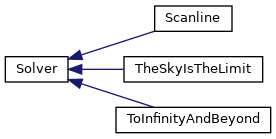
\includegraphics[scale=0.7]{img/solver_UML}
\caption{Diagramme UML de \texttt{Solver} et ses filles}
\label{fig:uml}
\end{figure}

Ces trois solveurs reposent d'ailleurs sur des rectangles enveloppant nos formes de bases, de manière à ne considérer que des rectangles lors du packing (ils sont donc plus efficaces pour des formes qui sont de base des rectangles).\\

On peut voir en figure~\ref{la banane} le résultat de l'exécution du troisième solveur, sur un carré arbitrairement découpé au préalable. On constate que les formes ainsi générées ont été packées en 3 plaques (les échelles étant différentes à gauche et à droite, une plaque faisant la taille de la forme originale).

\begin{figure}[htb!]
\center
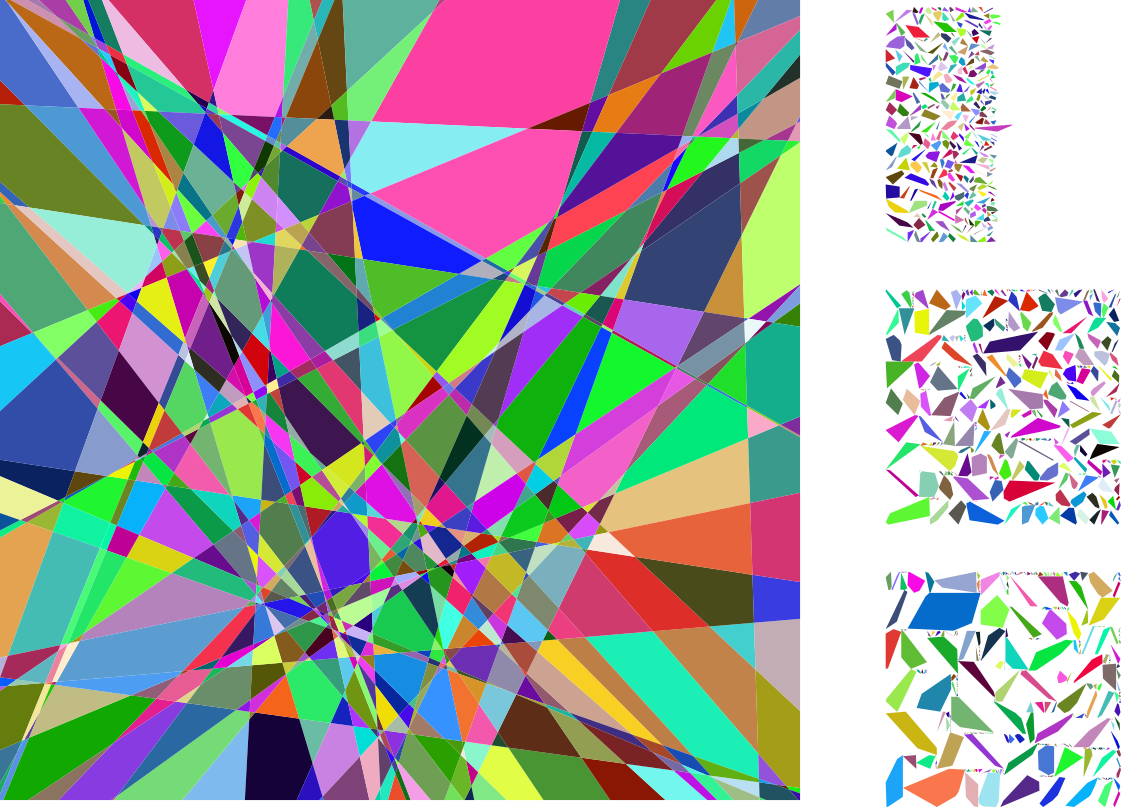
\includegraphics[scale=0.4]{img/scanLineTest}
\caption{Test du solveur "first-fit" ScanLineSolver}
\label{la banane}
\end{figure}



\newpage
\subsection{Outer}

La dernière étape de l'exécution a pour objectif d'écrire un fichier SVG contenant toutes les formes sélectionnées par l'utilisateur, après leur traitement par la classe \texttt{Solver}. Ceci est réalisé par la classe \texttt{Outer}, qui, à partir des formes précédemment déplacées par le \texttt{Solver} et de leurs identifiants récupérés par la classe \texttt{Parser}, va recopier les éléments associés à ces identifiants sur la sortie standard.\\

On parcourt donc l'arborescence du fichier SVG, en utilisant rapidXML, de manière à sélectionner les éléments en fonction de leur identifiant, pour ensuite ajouter (ou de modifier si le champ existe déjà) un champ contenant la matrice de transformation associée au déplacements effectués lors du packing.\\

Dans le cas d'une duplication (en bas de page), tous les éléments de l'arborescence parsés lors du parcours sont d'abord recopiés sans être modifiés, puis leur version modifiée est ajoutée si leur identifiant est reconnu comme élément à packer. On écrit ensuite sur la sortie standard le texte correspondant au fichier SVG ainsi généré, qui sera récupéré par le plugin ou par l'utilisateur pour être écrite dans un fichier.

